\documentclass[11pt]{article} 
\usepackage[english]{babel}
\usepackage[utf8]{inputenc}
\usepackage[margin=0.5in]{geometry}
\usepackage{amsmath}
\usepackage{amsthm}
\usepackage{amsfonts}
\usepackage{amssymb}
\usepackage[usenames,dvipsnames]{xcolor}
\usepackage{graphicx}
\usepackage[siunitx]{circuitikz}
\usepackage{tikz}
\usetikzlibrary{calc,arrows.meta}
\usepackage[colorinlistoftodos, color=orange!50]{todonotes}
\usepackage{hyperref}
\usepackage[numbers, square]{natbib}
\usepackage{fancybox}
\usepackage{epsfig}
\usepackage{soul}
\usepackage[framemethod=tikz]{mdframed}
\usepackage[shortlabels]{enumitem}
\usepackage[version=4]{mhchem}
\usepackage{multicol}

\usepackage{mathtools}
\usepackage{comment}
\usepackage{enumitem}
\usepackage[utf8]{inputenc}
\usepackage[linesnumbered,ruled,vlined]{algorithm2e}
\usepackage{listings}
\usepackage{color}
\usepackage[numbers]{natbib}
\usepackage{subfiles}
\usepackage{tkz-berge}


\newtheorem{prop}{Proposition}[section]
\newtheorem{thm}{Theorem}[section]
\newtheorem{lemma}{Lemma}[section]
\newtheorem{cor}{Corollary}[prop]

\theoremstyle{definition}
\newtheorem{definition}{Definition}

\theoremstyle{definition}
\newtheorem{required}{Problem}

\theoremstyle{definition}
\newtheorem{ex}{Example}

\tikzset{
	vertex/.style={circle,draw,minimum size=16, inner sep=0pt,font=\normalsize},
	every node/.style={draw=none,rectangle,font=\scriptsize,outer sep=0pt,inner sep=2pt},
	directed/.style={arrows={-Stealth[length=7pt]},font=\small},
	caption/.style={text width=6cm,align=center,rectangle,draw}
}


\setlength{\marginparwidth}{3.4cm}
%#########################################################

%To use symbols for footnotes
\renewcommand*{\thefootnote}{\fnsymbol{footnote}}
%To change footnotes back to numbers uncomment the following line
%\renewcommand*{\thefootnote}{\arabic{footnote}}

% Enable this command to adjust line spacing for inline math equations.
% \everymath{\displaystyle}

% _______ _____ _______ _      ______ 
%|__   __|_   _|__   __| |    |  ____|
%   | |    | |    | |  | |    | |__   
%   | |    | |    | |  | |    |  __|  
%   | |   _| |_   | |  | |____| |____ 
%   |_|  |_____|  |_|  |______|______|
%%%%%%%%%%%%%%%%%%%%%%%%%%%%%%%%%%%%%%%

\title{
\normalfont \normalsize 
\textsc{CSCI 3104 Fall 2021 \\ 
Instructors: Profs. Grochow and Waggoner} \\
[10pt] 
\rule{\linewidth}{0.5pt} \\[6pt] 
\huge Quiz- Standard 12 \\
\rule{\linewidth}{2pt}  \\[10pt]
}
%\author{Your Name}
\date{}

\begin{document}
\definecolor {processblue}{cmyk}{0.96,0,0,0}
\definecolor{processred}{rgb}{200, 0, 0}
\definecolor{processgreen}{rgb}{0, 255, 0}
\DeclareGraphicsExtensions{.png}
\DeclareGraphicsExtensions{.gif}
\DeclareGraphicsExtensions{.jpg}

\maketitle


%%%%%%%%%%%%%%%%%%%%%%%%%
%%%%%%%%%%%%%%%%%%%%%%%%%%
%%%%%%%%%%FILL IN YOUR NAME%%%%%%%
%%%%%%%%%%AND STUDENT ID%%%%%%%%
%%%%%%%%%%%%%%%%%%%%%%%%%%
\noindent
Due Date \dotfill TODO \\
Name \dotfill \textbf{Didi Trifonova} \\
Student ID \dotfill \textbf{109388776} \\


\tableofcontents

\section{Instructions}
 \begin{itemize}
	\item The solutions \textbf{should be typed}, using proper mathematical notation. We cannot accept hand-written solutions. \href{http://ece.uprm.edu/~caceros/latex/introduction.pdf}{Here's a short intro to \LaTeX.}
	\item You should submit your work through the \textbf{class Canvas page} only. Please submit one PDF file, compiled using this \LaTeX \ template.
	\item You may not need a full page for your solutions; pagebreaks are there to help Gradescope automatically find where each problem is. Even if you do not attempt every problem, please submit this document with no fewer pages than the blank template (or Gradescope has issues with it).

	\item You \textbf{may not collaborate with other students}. \textbf{Copying from any source is an Honor Code violation. Furthermore, all submissions must be in your own words and reflect your understanding of the material.} If there is any confusion about this policy, it is your responsibility to clarify before the due date. 

	\item Posting to \textbf{any} service including, but not limited to Chegg, Discord, Reddit, StackExchange, etc., for help on an assignment is a violation of the Honor Code.

	\item You \textbf{must} virtually sign the Honor Code (see Section \ref{HonorCode}). Failure to do so will result in your assignment not being graded.
\end{itemize}


\section{Honor Code (Make Sure to Virtually Sign)} \label{HonorCode}

\begin{required}
\noindent 
\begin{itemize}
\item My submission is in my own words and reflects my understanding of the material.
\item I have not collaborated with any other person.
\item I have not posted to external services including, but not limited to Chegg, Discord, Reddit, StackExchange, etc.
\item I have neither copied nor provided others solutions they can copy.
\end{itemize}

%\noindent In the specified region below, clearly indicate that you have upheld the Honor Code. Then type your name. 
\end{required}

\begin{proof}[Agreed (Didi Trifonova).]
I agree to the above
\end{proof}



\newpage
\section{Standard 12- Calculus I}

\begin{required} \label{Problem2}
Let $f(n) = n^{2}$ and $g(n) = 3n^{2} + 4n \log(n)$. Determine the relationship that \textbf{best} applies: $f(n) \in o(g(n))$, $f(n) \in O(g(n)), f(n) \in \Theta(g(n))$, $f(n) \in \omega(g(n))$, or $f(n) \in \Omega(g(n))$. Prove your answer. Note that you are expected to spell out \textbf{all Calculus details} at the level of Calculus I-II.
\begin{itemize}
\item Note that $f(n) \in o(g(n))$ means that $f(n) \in O(g(n))$, but that $f(n) \not \in \Theta(g(n))$.
\item Note that $f(n) \in \omega(g(n))$ means that $f(n) \in \Omega(g(n))$, but that $f(n) \not \in \Theta(g(n))$.
\end{itemize}
\end{required}

\begin{proof} $ f(n) \in \Theta(g(n))$ Work on next page\\
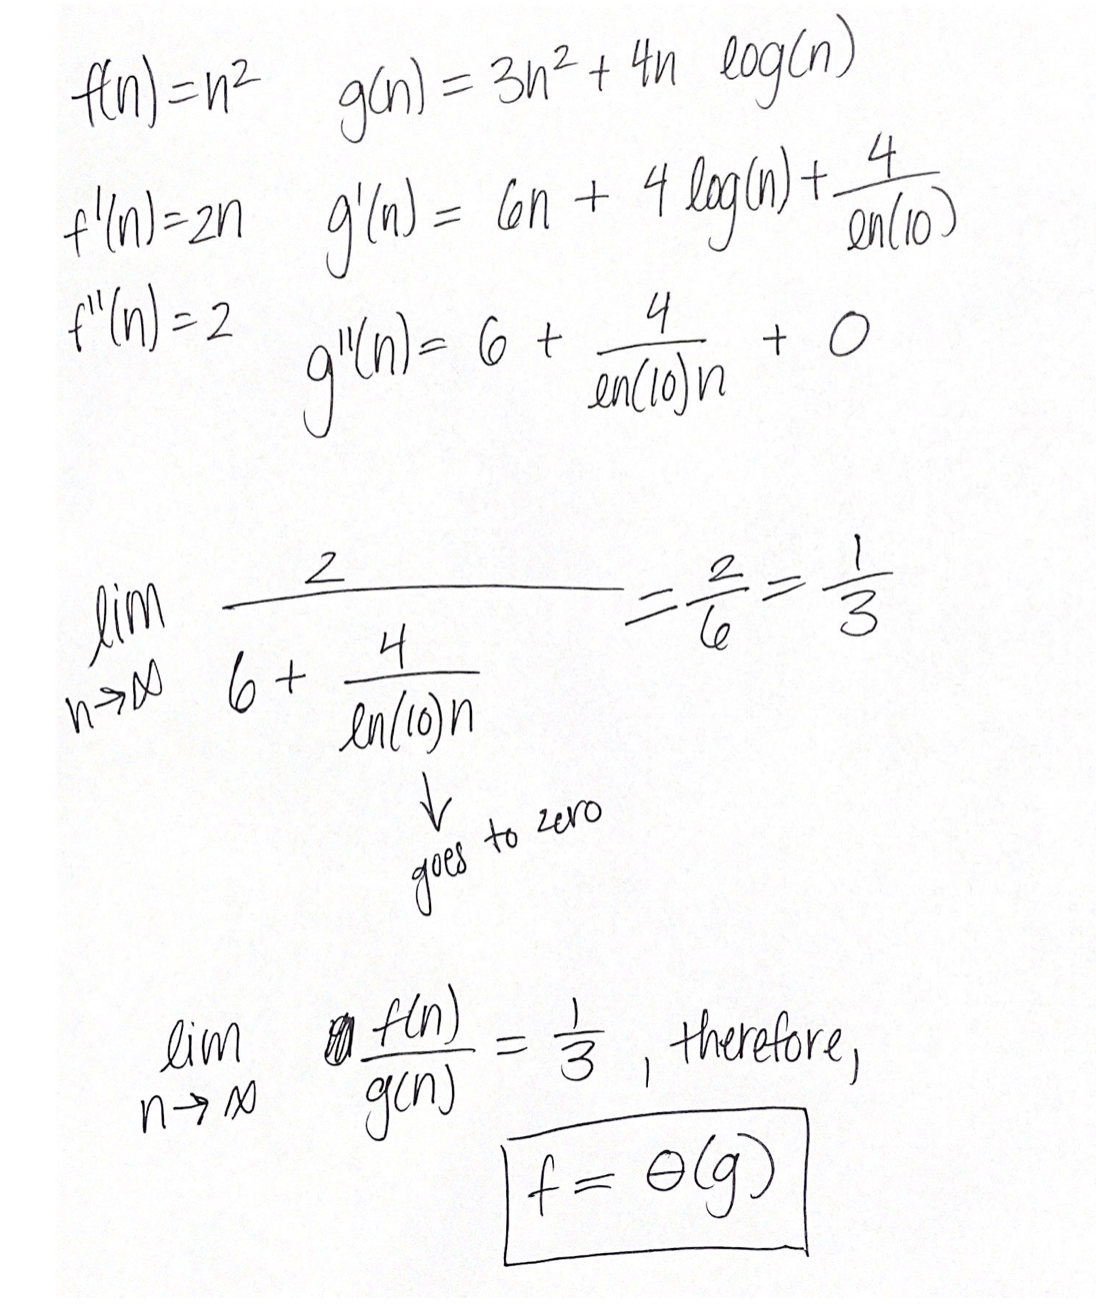
\includegraphics[]{answer.png}
\end{proof}


%Include an Image: \includegraphics{ImageFileName}
%Include an Image and Rotate 90 degree: \includegraphics[angle=90]{ImageFileName}
%Include an Image, Rotate by 180 degrees, and scale by 50\% \includegraphics[scale=0.5, angle=90]{ImageFileName}

%%%%%%%%%%%%%%%%%%%%%%%%%%%%%%%%%%%%%%%%%%%%%%%%%%
\end{document} % NOTHING AFTER THIS LINE IS PART OF THE DOCUMENT



